\section{Flag 06 - Admin (htpassword)}

\paragraph{d19b4823e0d5600ceed56d5e896ef328d7a2b9e7ac7e80f4fcdb9b10bcb3e7ff}
\begin{center}
    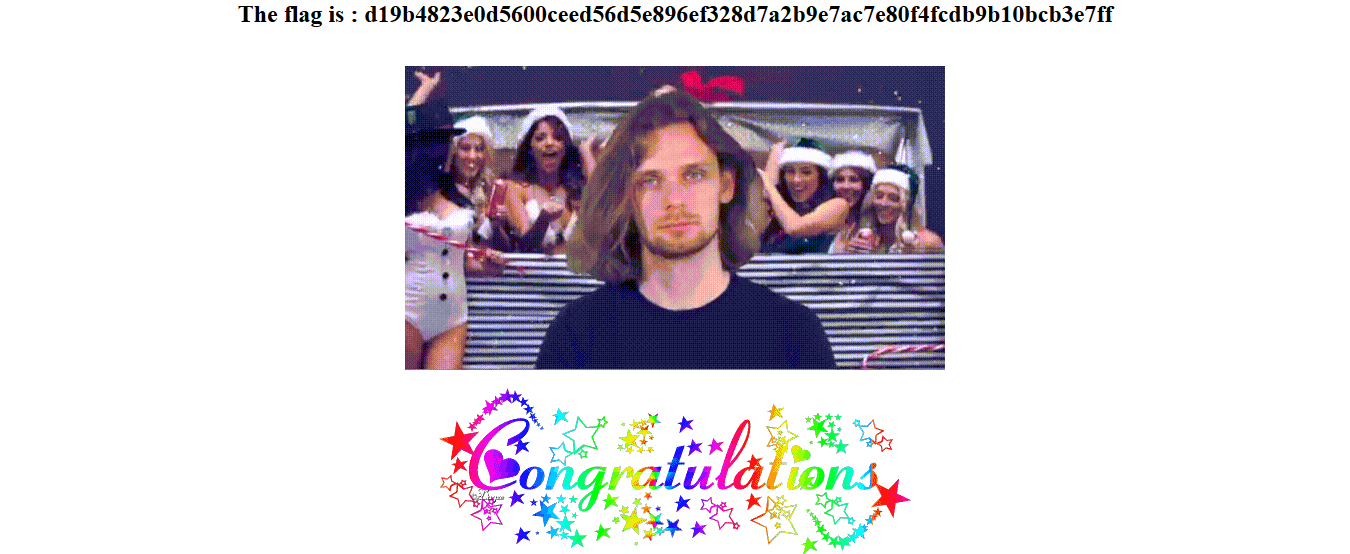
\includegraphics[width=0.5\textwidth]{09.Flag06/06-06.png}\\[0cm] 
\end{center}

\subsection{Vulnerability}

\begin{itemize}
    \item htpasswd is accessible.
    \item Storage of credentials on the server
    \item Using MD5 hash    
\end{itemize}

\subsection{Location}

\begin{itemize}
    \item 'http://<ip-address>:80/robots.txt'
    \item 'http://<ip-address>:80/whatever'
    \item 'http://<ip-address>:80/admin'
\end{itemize}

\subsection{Method}

The `robots.txt` file lists directories it does not allow to be indexed by 'Web Crawlers'. Access to these directories is not subsequently protected from access.

One of the directories listed is `whatever`. When one goes to `http://<ip-address>:80/whatever` they will see:

```

Index of /whatever/

../

htpasswd                                           13-Dec-2015 17:41                  38

```

Clicking on htpassword and opening the content with a text editor will reveal `root:8621ffdbc5698829397d97767ac13db3`. Entering the string `8621ffdbc5698829397d97767ac13db3` into \href{https://hashes.com/en/decrypt/hash}{hashes.com} will reveal it is MD5 hash of `dragon`.

You must then navigate to `http://<ip-address>:80/admin` and enter in the credententials `root` and `dragon`. This will log you in to an area with the flag.

\subsection{Tools}

\begin{figure}[!htb]
    \centering
    \subfloat[robots.txt]{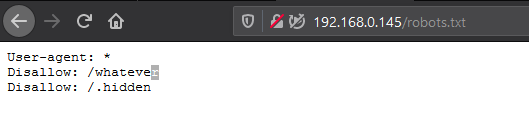
\includegraphics[width=.45\columnwidth]{09.Flag06/06-01.png}\label{fig: 06-01 - wtf}} \quad
    \subfloat[index of whatever]{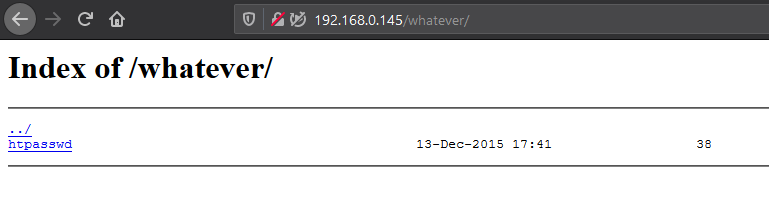
\includegraphics[width=.45\columnwidth]{09.Flag06/06-02.png}\label{fig: 06-02 - wrong}} \\
    \subfloat[htpasswd]{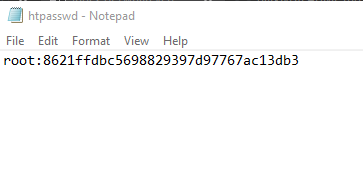
\includegraphics[width=.45\columnwidth]{09.Flag06/06-03.png}\label{fig: 06-03 - nope}} \quad
    \subfloat[hashes.com]{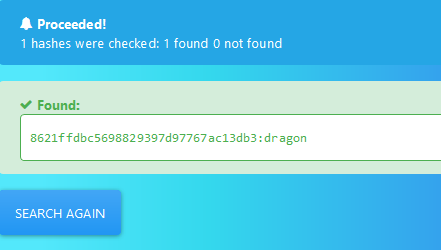
\includegraphics[width=.45\columnwidth]{09.Flag06/06-04.png}\label{fig: 06-04 - wrong}} \\
    \subfloat[admin login area]{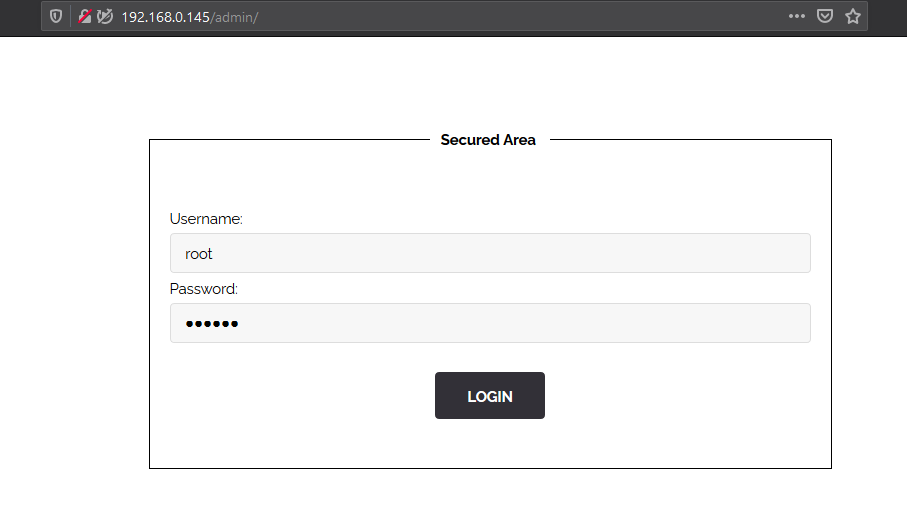
\includegraphics[width=.45\columnwidth]{09.Flag06/06-05.png}\label{fig: 06-05 - nope}} \quad
    \caption[Flag 06 Method]{Process to Capture the Admin Flag} % The text in the square bracket is the caption for the list of figures while the text in the curly brackets is the figure caption
    \label{fig:flag06 method}
\end{figure}

\begin{itemize}
    \item \href{https://www.reddit.com/r/HowToHack/comments/2030df/find_hidden_files_on_a_website/}{Reddit - How to Hack}
    \item \href{https://en.wikipedia.org/wiki/Directory\_traversal\_attack}{Wikipedia - Directory Traversal Attack}
    \item \href{https://nmap.org/nsedoc/scripts/http-enum.html}{Nmap - Enum}
    \item \href{https://towardsdatascience.com/web-scraping-using-selenium-python-8a60f4cf40ab}{Selenium - Web Scraper}
    \item \href{https://support.google.com/webmasters/answer/6062608?hl=en}{Google - Introduction to robots.txt}
    \item \href{https://tools.kali.org/web-applications/dirbuster}{OWASP DirBuster}
    \item \href{https://hashes.com/en/decrypt/hash}{hashes.com}
\end{itemize}

\subsection{Remedy}

\begin{itemize}
    \item Do not store \textbf{Credentials} on \textbf{SERVER}
    \item Disallow direct access to directories
\end{itemize}
